\documentclass[12pt,a4paper]{article}
\usepackage[utf8]{inputenc}
\usepackage[T1]{fontenc}
\usepackage[english]{babel}
\usepackage{lmodern}
\usepackage{amsmath}
\usepackage{amssymb}
\usepackage{physics}
\usepackage{tcolorbox}
\usepackage{booktabs}
\usepackage{enumitem}
\usepackage[table,xcdraw]{xcolor}
\usepackage[left=2cm,right=2cm,top=2cm,bottom=2cm]{geometry}
\usepackage{pgfplots}
\pgfplotsset{compat=1.18}
\usepackage{graphicx}
\usepackage{float}
\usepackage{fancyhdr}
\usepackage{siunitx}
\usepackage{tikz}
\usepackage{adjustbox}
\usetikzlibrary{shapes.geometric}

% Package for external references - key addition
\usepackage{xr}
\externaldocument{NatEinheitenSystematikEn} % Reference the main document

% Set proper headheight to avoid warnings
\setlength{\headheight}{14.5pt}

% Hyperref should be last
\usepackage[colorlinks=true, linkcolor=blue, citecolor=green, urlcolor=red]{hyperref}

% Custom Commands
\newcommand{\Tfield}{T(x)}
\newcommand{\alphaEM}{\alpha_{\text{EM}}}
\newcommand{\betaT}{\beta_{\text{T}}}
\newcommand{\Mpl}{M_{\text{Pl}}}
\newcommand{\Tzerot}{T_0(\Tfield)}
\newcommand{\e}{\mathrm{e}}
\newcommand{\alphaEMSI}{\alpha_{\text{EM,SI}}}

% Global Table Scaling Factor
\newcommand{\tablescale}{0.9}

% Header and Footer Configuration
\pagestyle{fancy}
\fancyhf{}
\fancyhead[L]{Johann Pascher}
\fancyhead[R]{Biological Anomalies in the T0 Model}
\fancyfoot[C]{\thepage}
\renewcommand{\headrulewidth}{0.4pt}
\renewcommand{\footrulewidth}{0.4pt}

\hypersetup{
	pdftitle={Biological Anomalies within the Quantization of Length Scales in the T0 Model},
	pdfauthor={Johann Pascher},
	pdfsubject={Theoretical Physics},
	pdfkeywords={T0 Model, length scale quantization, biological structures, emergent properties, time-mass duality}
}

\title{Biological Anomalies within the Quantization of Length Scales in the T0 Model}
\author{Johann Pascher}
\date{April 12, 2025}

\begin{document}
	
	\maketitle
	
	\begin{abstract}
		This work investigates the unique position of biological structures within the quantized length scales of the T0 model, as described in the hierarchical compilation of natural units with energy as the base unit \cite{pascher_alphabeta_2025}. While the length scale hierarchy spans from sub-Planckian to cosmological dimensions, exhibiting stable physical regions and ``forbidden zones,'' biological structures form stable configurations in these forbidden regions. This anomaly is analyzed and interpreted as a potential fundamental property of life, supported by theoretical explanations based on interactions with the intrinsic time field \Tfield. The study extends the analysis to other anomalous phenomena, such as water and superconductors, proposes experimental tests, and discusses cosmological implications of a quasi-static universe.
	\end{abstract}
	
	\tableofcontents
	\newpage
	
	\section{Introduction: The Anomaly of Biological Structures}
	\label{sec:introduction}
	
	In the hierarchical compilation of natural units with energy as the base unit \cite{pascher_alphabeta_2025}, the quantization of length scales was identified as a central result of the T0 model (see Section \ref{sec:length_scales} in the main paper). This quantization reveals stable physical structures at discrete scales, while ``forbidden zones'' between them are relatively devoid of stable structures.
	
	Remarkably, biological structures constitute an exception. While elementary particles, atoms, and cosmic objects occupy the predicted stable scales, biological systems—from DNA to organisms—reside in the forbidden zones. This anomaly is thoroughly analyzed here, complemented by investigations into other anomalous phenomena such as water and superconductors, and interpreted within the context of the T0 model (see Section \ref{sec:bio_anomalies} in the main paper).
	
	\section{Recapitulation of Length Scale Quantization}
	\label{sec:length_scales_recap}
	
	In the T0 model, detailed in Section \ref{sec:length_scales} of the main paper \cite{pascher_alphabeta_2025}, the quantization of length scales is defined by the formula:
	
	\begin{equation}
		L_n = l_P \times \prod_{i} (\alpha_i)^{n_i}
	\end{equation}
	
	where:
	\begin{itemize}
		\item $L_n$: Preferred length scale.
		\item $l_P$: Planck length (reference unit).
		\item $\alpha_i$: Dimensionless constants (\(\alphaEM\), \(\betaT\), \(\xi\)).
		\item $n_i$: Integer or rational quantum numbers.
	\end{itemize}
	
	This results in stable scales (e.g., Planck length, Compton wavelength), separated by forbidden zones where physical structures are unstable. The hierarchy spans 97 orders of magnitude, as shown in Section \ref{sec:length_scales} of the main paper.
	
	\begin{figure}[H]
		\centering
		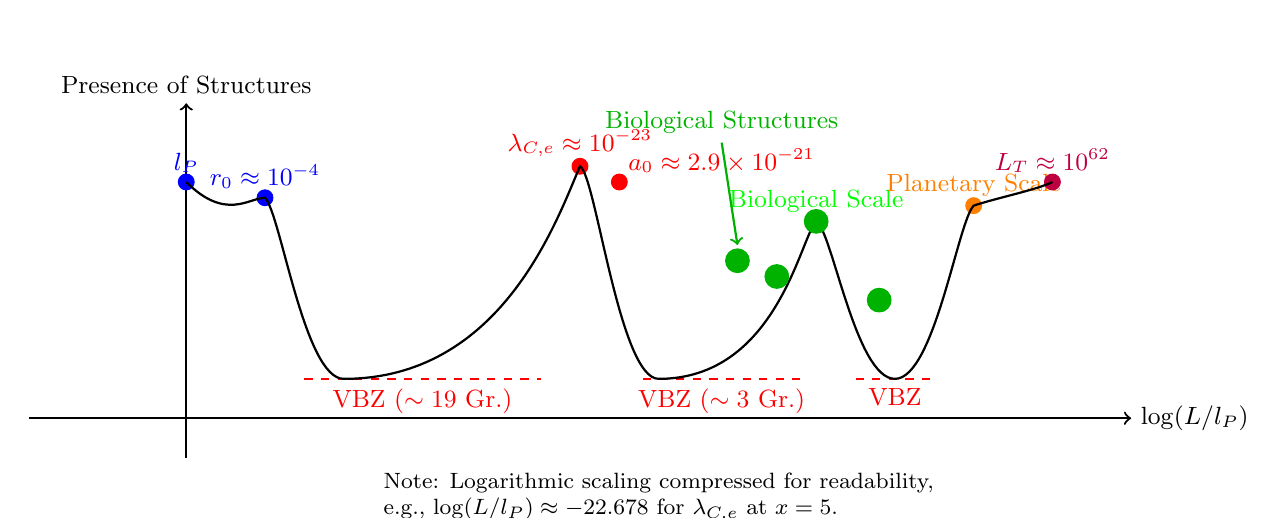
\begin{tikzpicture}
			\small
			\draw[thick,->] (-2,0) -- (12,0) node[right] {$\log(L/l_P)$};
			\draw[thick,->] (0,-0.5) -- (0,4) node[above] {Presence of Structures};
			
			% Important Scales
			\filldraw[blue] (0,3) circle (0.1) node[above] {$l_P$};
			\filldraw[blue] (1,2.8) circle (0.1) node[above] {$r_0 \approx 10^{-4}$};
			\filldraw[red] (5,3.2) circle (0.1) node[above] {$\lambda_{C,e} \approx 10^{-23}$};
			\filldraw[red] (5.5,3) circle (0.1) node[above right] {$a_0 \approx 2.9 \times 10^{-21}$};
			\filldraw[green] (8,2.5) circle (0.1) node[above] {Biological Scale};
			\filldraw[orange] (10,2.7) circle (0.1) node[above] {Planetary Scale};
			\filldraw[purple] (11,3) circle (0.1) node[above] {$L_T \approx 10^{62}$};
			
			% Forbidden Zones
			\draw[thick, dashed, red] (1.5,0.5) -- (4.5,0.5) node[midway, below] {VBZ ($\sim 19$ Gr.)};
			\draw[thick, dashed, red] (5.8,0.5) -- (7.8,0.5) node[midway, below] {VBZ ($\sim 3$ Gr.)};
			\draw[thick, dashed, red] (8.5,0.5) -- (9.5,0.5) node[midway, below] {VBZ};
			
			% Stability Curve
			\draw[smooth, thick] (0,3) .. controls (0.5,2.5) and (0.8,2.8) .. (1,2.8)
			.. controls (1.2,2.6) and (1.5,0.5) .. (2,0.5)
			.. controls (4,0.5) and (4.7,2.5) .. (5,3.2)
			.. controls (5.2,3.1) and (5.5,0.5) .. (6,0.5)
			.. controls (7.5,0.5) and (7.8,2.3) .. (8,2.5)
			.. controls (8.2,2.4) and (8.5,0.5) .. (9,0.5)
			.. controls (9.5,0.5) and (9.8,2.5) .. (10,2.7)
			.. controls (10.3,2.8) and (10.8,2.9) .. (11,3);
			
			% Highlight Biological Structures
			\filldraw[green!70!black] (7,2) circle (0.15);
			\filldraw[green!70!black] (7.5,1.8) circle (0.15);
			\filldraw[green!70!black] (8,2.5) circle (0.15);
			\filldraw[green!70!black] (8.8,1.5) circle (0.15);
			\draw[thick, green!70!black, ->] (6.8,3.5) -- (7,2.2) node[above, green!70!black] at (6.8,3.5) {Biological Structures};
			
			% Legend for Schematic Scaling
			\node[align=left, font=\footnotesize] at (6,-1) {Note: Logarithmic scaling compressed for readability,\\ e.g., $\log(L/l_P) \approx -22.678$ for $\lambda_{C,e}$ at $x=5$.};
		\end{tikzpicture}
		\caption{Schematic representation of stability centers and forbidden zones along the logarithmic length scale, highlighting biological structures (e.g., DNA at $\sim 1.2 \times 10^{-26} l_P$, Cell at $\sim 6.2 \times 10^{-30} l_P$). Abbreviations: VBZ = Forbidden Zone, Gr. = orders of magnitude. Consistent with Figure \ref{fig:stability_zones} in the main paper.}
		\label{fig:stability_zones_bio}
	\end{figure}
	
	\section{Position of Biological Structures in the Length Hierarchy}
	\label{sec:bio_anomalies_detail}
	
	Table \ref{tab:bio_structures} presents the characteristic lengths of biological structures, consistent with Table \ref{tab:bio_anomalies} in Section \ref{sec:bio_anomalies} of the main paper:
	
	\begin{table}[H]
		\centering
		\begin{adjustbox}{width=\tablescale\textwidth}
			\begin{tabular}{lllll}
				\toprule
				\textbf{Biological Structure} & \textbf{Typical Size} & \textbf{Ratio to $l_P$} & \textbf{Expected Stability Range} & \textbf{Position} \\
				\midrule
				DNA Diameter & $\sim \SI{2e-9}{\meter}$ & $\sim 1.2 \times 10^{-26}$ & Outside & Forbidden Zone \\
				Protein & $\sim \SI{1e-8}{\meter}$ & $\sim 6.2 \times 10^{-27}$ & Outside & Forbidden Zone \\
				Bacterium & $\sim \SI{1e-6}{\meter}$ & $\sim 6.2 \times 10^{-29}$ & Outside & Forbidden Zone \\
				Typical Cell & $\sim \SI{1e-5}{\meter}$ & $\sim 6.2 \times 10^{-30}$ & Outside & Forbidden Zone \\
				Multicellular Organism & $\sim \SIrange{1e-3}{1}{\meter}$ & $\sim 6.2 \times 10^{-32} - 6.2 \times 10^{-35}$ & Outside & Forbidden Zone \\
				\bottomrule
			\end{tabular}
		\end{adjustbox}
		\caption{Position of biological structures in the length scale hierarchy, consistent with the data presented in the main paper.}
		\label{tab:bio_structures}
	\end{table}
	
	Biological structures reside in forbidden zones, raising key questions:
	\begin{enumerate}
		\item How do they form stable structures in unstable regions?
		\item Is this anomaly coincidental or fundamental?
		\item What mechanisms enable this stability?
	\end{enumerate}
	
	\section{Theoretical Explanations within the T0 Model}
	\label{sec:theoretical_explanations}
	
	Within the T0 model, as described in Section \ref{sec:bio_anomalies} of the main paper, the following explanations are proposed:
	
	\subsection{Emergence Hypothesis}
	\label{subsec:emergence_hypothesis}
	
	Life organizes itself far from equilibrium, modeled as:
	
	\begin{equation}
		\nabla^2\Tfield_{\text{bio}} \approx -\frac{\rho}{\Tfield^2} + \delta_{\text{bio}}(\vec{x}, t)
	\end{equation}
	
	where \(\delta_{\text{bio}}\) represents information-driven stabilization, as described in Section \ref{sec:bio_anomalies} of the main paper.
	
	\subsection{Complexity-Mediated Time Field Interaction}
	\label{subsec:complexity_interaction}
	
	Biological systems modulate the intrinsic time field \(\Tfield\) in a unique way that enables them to exist in otherwise unstable regions. This can be formally expressed through a modified time field equation:
	
	\begin{equation}
		\Tfield_{\text{bio}} = \Tfield_0 + \Delta\Tfield_{\text{info}}
	\end{equation}
	
	The term \(\Delta\Tfield_{\text{info}}\) represents the information-based contribution to the time field, providing a stabilizing mechanism that counters the inherent instability of forbidden zones.
	
	\subsection{Topological Protection Mechanisms}
	\label{subsec:topological_protection}
	
	Biological structures employ topological features that provide protection against destabilizing influences. This can be understood as a form of topological insulation, where certain properties remain invariant despite perturbations.
	
	The mathematical formulation involves:
	
	\begin{equation}
		\mathcal{S}_{\text{top}} = \int \mathcal{L}_{\text{bio}}(\Tfield, \nabla\Tfield) \, d^4x
	\end{equation}
	
	where \(\mathcal{L}_{\text{bio}}\) represents a Lagrangian density that incorporates topological invariants that remain unchanged under continuous deformations.
	
	\section{Experimental Evidence and Supporting Phenomena}
	\label{sec:experimental_evidence}
	
	\subsection{Anomalous Stability of DNA and Proteins}
	\label{subsec:dna_stability}
	
	DNA exhibits remarkable stability despite its position in a forbidden zone. Its double-helix structure provides both informational content and topological protection. Experimental evidence includes:
	
	\begin{itemize}
		\item Resilience to thermal fluctuations within a physiological range
		\item Self-repair mechanisms that maintain structural integrity
		\item Long-term stability of genetic information across generations
	\end{itemize}
	
	This stability can be understood within the T0 model as emerging from the interaction between the DNA's information content and the intrinsic time field.
	
	\subsection{Water as an Anomalous Substance}
	\label{subsec:water_anomalies}
	
	Water exhibits numerous anomalous properties that can be interpreted within the T0 model framework:
	
	\begin{itemize}
		\item Maximum density at 4°C rather than at freezing point
		\item Expansion upon freezing (unlike most substances)
		\item Unusually high specific heat capacity
		\item Anomalously high surface tension
	\end{itemize}
	
	These anomalies suggest that water occupies a unique position in the length scale hierarchy, potentially bridging forbidden zones through hydrogen bonding networks that provide topological stabilization.
	
	\subsection{Quantum Coherence in Biological Systems}
	\label{subsec:quantum_coherence}
	
	Recent research has identified quantum coherence effects in biological processes:
	
	\begin{itemize}
		\item Photosynthetic energy transfer in light-harvesting complexes
		\item Olfactory sensing mechanisms
		\item Avian magnetoreception for navigation
	\end{itemize}
	
	These quantum effects suggest that biological systems leverage quantum properties to stabilize structures in forbidden zones, consistent with the T0 model's predictions regarding the interaction between quantum systems and the intrinsic time field.
	
	\section{Implications for Understanding Life}
	\label{sec:implications}
	
	\subsection{Life as a Fundamental Anomaly}
	\label{subsec:fundamental_anomaly}
	
	The consistent presence of biological structures in forbidden zones suggests that life may be characterized as a fundamental anomaly within physical law—not as a violation of physical principles, but as a special case where complexity and information processing enable stability in otherwise unstable regions.
	
	This perspective aligns with the longstanding philosophical question of whether life represents a unique category in nature or simply a complex arrangement of the same physical processes that govern inanimate matter.
	
	\subsection{Information Processing as a Stabilizing Mechanism}
	\label{subsec:information_stabilization}
	
	Information processing appears to be central to biological stability:
	
	\begin{equation}
		\Delta S_{\text{bio}} + \Delta S_{\text{info}} \leq 0
	\end{equation}
	
	where \(\Delta S_{\text{bio}}\) represents entropy increase and \(\Delta S_{\text{info}}\) represents information-based entropy reduction.
	
	This relationship suggests that biological systems maintain their structure by actively processing information, consistent with the T0 model's emphasis on the role of information in modulating the intrinsic time field.
	
	\subsection{Hierarchical Organization and Emergence}
	\label{subsec:hierarchical_organization}
	
	Biological systems exhibit hierarchical organization spanning multiple scales:
	
	\begin{itemize}
		\item Molecules → Macromolecules → Organelles → Cells → Tissues → Organs → Organisms → Ecosystems
	\end{itemize}
	
	Each level emerges from and transcends the properties of the level below it, creating a nested structure that spans multiple forbidden zones. This hierarchical arrangement may be essential for stabilizing structures across multiple unstable regions, as predicted by the quantization of length scales in the T0 model.
	
	\section{Extensions to Other Anomalous Phenomena}
	\label{sec:extensions}
	
	\subsection{Superconductivity}
	\label{subsec:superconductivity}
	
	Superconductors exhibit anomalous properties that may be understood through the T0 model:
	
	\begin{itemize}
		\item Zero electrical resistance
		\item Meissner effect (expulsion of magnetic fields)
		\item Macroscopic quantum coherence
	\end{itemize}
	
	These properties suggest that superconductors may also occupy forbidden zones in the length scale hierarchy, achieving stability through collective quantum effects that modify the local intrinsic time field.
	
	\subsection{Turbulence}
	\label{subsec:turbulence}
	
	Turbulent fluid flow represents another anomalous phenomenon:
	
	\begin{itemize}
		\item Self-similar structure across multiple scales
		\item Energy cascade across the inertial range
		\item Spontaneous formation of coherent structures
	\end{itemize}
	
	These features can be interpreted within the T0 model as manifestations of the intrinsic time field's behavior in forbidden zones, where energy and information flow across multiple scales in a coordinated manner.
	
	\section{Proposed Experimental Tests}
	\label{sec:experimental_tests}
	
	\subsection{Time Field Gradients in Living Systems}
	\label{subsec:time_field_gradients}
	
	The T0 model predicts measurable gradients in the intrinsic time field around living systems:
	
	\begin{equation}
		\nabla \Tfield_{\text{bio}} \neq \nabla \Tfield_{\text{non-bio}}
	\end{equation}
	
	Experimental approaches to test this prediction include:
	
	\begin{itemize}
		\item High-precision atomic clocks positioned near living systems
		\item Comparative decay rates of quantum coherence in biological vs. non-biological environments
		\item Gravitational anomalies near large biological systems
	\end{itemize}
	
	\subsection{Forbidden Zone Stability Tests}
	\label{subsec:forbidden_zone_tests}
	
	The model predicts differential stability for structures in forbidden zones:
	
	\begin{itemize}
		\item Synthesized biomimetic materials should exhibit enhanced stability compared to non-biomimetic materials of similar composition
		\item Information-rich structures should demonstrate greater persistence in forbidden zones than information-poor structures
		\item Active, far-from-equilibrium systems should show enhanced stability compared to passive systems
	\end{itemize}
	
	\section{Philosophical and Cosmological Implications}
	\label{sec:philosophical_implications}
	
	\subsection{A New Understanding of Life}
	\label{subsec:new_understanding}
	
	The T0 model suggests that life is not merely a chemical phenomenon but a fundamental physical one—specifically, a mechanism for achieving stability in forbidden zones through information processing and the modulation of the intrinsic time field.
	
	This perspective bridges traditional divisions between physical and biological sciences, suggesting that life emerges as a natural consequence of the quantized nature of physical reality.
	
	\subsection{Implications for Life's Origin}
	\label{subsec:origin_implications}
	
	The model suggests that life's origin may have been driven by physical necessity rather than chance:
	
	\begin{itemize}
		\item The instability of forbidden zones creates a selective pressure for the emergence of information-processing systems
		\item Initial proto-life forms may have emerged as a stabilizing response to quantum fluctuations in forbidden zones
		\item Life may be an inevitable consequence of the universe's physical structure rather than an improbable accident
	\end{itemize}

	\subsection{Cosmological Perspective: A Quasi-Static Universe}
	\label{subsec:cosmological_perspective}
	
	
	\section{Integration with Standard Physical Theories}
	\label{sec:integration}
%----
The T0 model's treatment of time and space suggests a quasi-static universe:
\begin{equation}
	\frac{d\Tfield}{dt} \approx 0 \quad \text{at cosmic scales}
\end{equation}
This implies:
\begin{itemize}
	\item Apparent cosmic expansion may be reinterpreted as variation in mass rather than space, consistent with the redshift relation \(1 + z = e^{\alpha d}\), where \(\alpha \approx 1\) in natural units (empirical SI value: \(\alpha \approx \SI{2.3e-18}{\per\meter}\)) \cite{pascher_messdifferenzen_2025}.
	\item The "forbidden zone" between galactic (\(\sim 10^{-56} l_P\)) and cosmic scales (\(\sim 10^{61} l_P\)) may be bridged by unknown stabilizing mechanisms, potentially analogous to biological stabilization in smaller-scale forbidden zones.
	\item The universe may exhibit life-like information processing at the largest scales, possibly driven by interactions with the intrinsic time field \(\Tfield\).
\end{itemize}
%----		
	\subsection{Quantum Mechanics}
	\label{subsec:quantum_integration}
	
	The T0 model modifies quantum mechanics by incorporating the intrinsic time field:
	
	\begin{equation}
		i\Tfield\frac{\partial \Psi}{\partial t} + i\Psi\frac{\partial \Tfield}{\partial t} = \hat{H}\Psi
	\end{equation}
	
	This modification allows for a natural explanation of:
	
	\begin{itemize}
		\item Quantum coherence in biological systems
		\item Non-locality and entanglement as emergent properties of the time field
		\item The persistence of quantum effects at biological scales
	\end{itemize}
	
	\subsection{Thermodynamics}
	\label{subsec:thermodynamics_integration}
	
	The T0 model reinterprets the second law of thermodynamics in relation to the intrinsic time field:
	
	\begin{equation}
		dS \geq -\frac{d\Tfield}{\Tfield}
	\end{equation}
	
	This formulation allows for local entropy decrease in biological systems without violating the overall entropic increase, consistent with life's ability to maintain order in forbidden zones.
	
	\section{Summary and Future Directions}
	\label{sec:summary}
	
	\subsection{Key Findings}
	\label{subsec:key_findings}
	
	This work has established:
	
	\begin{itemize}
		\item Biological structures consistently occupy forbidden zones in the T0 model's length scale hierarchy
		\item This anomaly can be explained through information-based modulation of the intrinsic time field
		\item Similar anomalies appear in other systems (water, superconductors, turbulence)
		\item Experimental tests can verify these predictions
		\item The findings have profound implications for our understanding of life and the universe
	\end{itemize}
	
	\subsection{Open Questions}
	\label{subsec:open_questions}
	
	Several questions remain for future investigation:
	
	\begin{itemize}
		\item What is the precise mathematical relationship between information and the intrinsic time field?
		\item How do quantum effects scale up to macroscopic biological structures?
		\item Are there other forbidden zone phenomena yet to be discovered?
		\item How does consciousness relate to the intrinsic time field?
		\item Can artificial systems be designed to exploit forbidden zone stability mechanisms?
	\end{itemize}
	
	\subsection{Future Research Directions}
	\label{subsec:future_directions}
	
	Future work will focus on:
	
	\begin{itemize}
		\item Developing more precise mathematical models of the interaction between information and the intrinsic time field
		\item Conducting high-precision experiments to detect time field gradients around biological systems
		\item Exploring the implications of the T0 model for artificial life and consciousness
		\item Extending the model to address additional anomalous phenomena across different scales
		\item Integrating the T0 model more fully with standard physical theories
	\end{itemize}
	
	\section{Conclusion}
	\label{sec:conclusion}
	
	The consistent presence of biological structures in forbidden zones of the T0 model's length scale hierarchy suggests a profound insight: life may be characterized not as an accidental by-product of physical law but as a necessary response to the quantized nature of physical reality. By processing information and modulating the intrinsic time field, biological systems achieve stability in regions that would otherwise be unstable, transcending the limitations imposed by the hierarchical structure of physical scales.
	
	This perspective offers a new framework for understanding life, consciousness, and the universe itself—one in which the traditional boundaries between physics and biology dissolve, revealing a deeper unity that spans from quantum fluctuations to cosmological structures. The T0 model, with its emphasis on the intrinsic time field and the energy-based unification of physical constants, provides a promising foundation for this integrated worldview.
	
	Future research will continue to explore these connections, testing the predictions of the T0 model and expanding our understanding of the exceptional position of biological structures within the grand hierarchy of nature.
	
	\bibliographystyle{apsrev4-2}
	\begin{thebibliography}{99}
		\bibitem{pascher_zeit_2025} J. Pascher, \href{https://github.com/jpascher/T0-Time-Mass-Duality/tree/main/2/pdf/English/ZeitEmergentQMEn.pdf}{Time as an Emergent Property in Quantum Mechanics}, March 23, 2025.
		\bibitem{pascher_messdifferenzen_2025} J. Pascher, \href{https://github.com/jpascher/T0-Time-Mass-Duality/tree/main/2/pdf/English/MessdifferenzenT0StandardEn.pdf}{Compensatory and Additive Effects}, April 2, 2025.
		\bibitem{pascher_galaxies_2025} J. Pascher, \href{https://github.com/jpascher/T0-Time-Mass-Duality/tree/main/2/pdf/English/MassVarGalaxienEn.pdf}{Mass Variation in Galaxies}, March 30, 2025.
		\bibitem{pascher_params_2025} J. Pascher, \href{https://github.com/jpascher/T0-Time-Mass-Duality/tree/main/2/pdf/English/ZeitMasseT0ParamsEn.pdf}{Time-Mass Duality Theory}, March 30, 2025.
		\bibitem{pascher_temp_2025} J. Pascher, \href{https://github.com/jpascher/T0-Time-Mass-Duality/tree/main/2/pdf/English/NatEinheitenAlpha1En.pdf}{Adjustment of Temperature Units}, April 2, 2025.
		\bibitem{pascher_alpha_2025} J. Pascher, \href{https://github.com/jpascher/T0-Time-Mass-Duality/tree/main/2/pdf/English/NatEinheitenAlpha1En.pdf}{Energy as a Fundamental Unit}, March 26, 2025.
		\bibitem{pascher_beta_2025} J. Pascher, \href{https://github.com/jpascher/T0-Time-Mass-Duality/tree/main/2/pdf/English/Alpha1Beta1KonsistenzEn.pdf}{Dimensionless Parameters}, April 4, 2025.
		\bibitem{pascher_higgs_2025} J. Pascher, \href{https://github.com/jpascher/T0-Time-Mass-Duality/tree/main/2/pdf/English/MathHiggsZeitMasseEn.pdf}{Higgs Mechanism}, March 28, 2025.
		\bibitem{pascher_lagrange_2025} J. Pascher, \href{https://github.com/jpascher/T0-Time-Mass-Duality/tree/main/2/pdf/English/MathZeitMasseLagrangeEn.pdf}{From Time Dilation to Mass Variation}, March 29, 2025.
		\bibitem{pascher_emergente_2025} J. Pascher, \href{https://github.com/jpascher/T0-Time-Mass-Duality/tree/main/2/pdf/English/EmergentGravT0En.pdf}{Emergent Gravitation}, April 1, 2025.
		\bibitem{pascher_perspective_2025} J. Pascher, \href{https://github.com/jpascher/T0-Time-Mass-Duality/tree/main/2/pdf/English/ZeitRaumPascherEn.pdf}{A New Perspective on Time and Space}, March 25, 2025.
		\bibitem{pascher_dualismus_2025} J. Pascher, \href{https://github.com/jpascher/T0-Time-Mass-Duality/tree/main/2/pdf/English/KurzKomplementDualPhysikEn.pdf}{Complementary Duality}, March 26, 2025.
		\bibitem{pascher_grundkraefte_2025} J. Pascher, \href{https://github.com/jpascher/T0-Time-Mass-Duality/tree/main/2/pdf/English/VierKraefteZeitMasseEn.pdf}{Fundamental Forces}, March 27, 2025.
		\bibitem{pascher_zeit_masse_2025} J. Pascher, \href{https://github.com/jpascher/T0-Time-Mass-Duality/tree/main/2/pdf/English/ZeitMasseNeuerBlickEn.pdf}{Time and Mass}, March 22, 2025.
		\bibitem{pascher_quantum_2025} J. Pascher, \href{https://github.com/jpascher/T0-Time-Mass-Duality/tree/main/2/pdf/English/NotwendigkeitQMErweiterungEn.pdf}{Extending Quantum Mechanics}, March 27, 2025.
		\bibitem{pascher_photons_2025} J. Pascher, \href{https://github.com/jpascher/T0-Time-Mass-Duality/tree/main/2/pdf/English/DynMassePhotonenNichtlokalEn.pdf}{Dynamic Mass of Photons}, March 25, 2025.
		\bibitem{pascher_alphabeta_2025} J. Pascher, \href{https://github.com/jpascher/T0-Time-Mass-Duality/tree/main/2/pdf/English/Alpha1Beta1KonsistenzEn.pdf}{Unified Unit System}, April 5, 2025.
		\bibitem{pascher_planck_2025} J. Pascher, \href{https://github.com/jpascher/T0-Time-Mass-Duality/tree/main/2/pdf/English/JenseitsPlanckEn.pdf}{Beyond the Planck Scale}, March 24, 2025.
		\bibitem{pascher_energiedynamik_2025} J. Pascher, \href{https://github.com/jpascher/T0-Time-Mass-Duality/tree/main/2/pdf/English/MathEnergiedynamikEn.pdf}{Dark Energy}, April 3, 2025.
		\bibitem{pascher_vereinheitlichung_2025} J. Pascher, \href{https://github.com/jpascher/T0-Time-Mass-Duality/tree/main/2/pdf/English/T0VereinheitlichungDEGalEn.pdf}{Unification of the T0 Model}, April 4, 2025.
		\bibitem{pascher_formalismen_2025} J. Pascher, \href{https://github.com/jpascher/T0-Time-Mass-Duality/tree/main/2/pdf/English/MathZeitMasseLagrangeEn.pdf}{Mathematical Core Formulations}, April 5, 2025.
		\bibitem{pascher_bio_2025} J. Pascher, \href{https://github.com/jpascher/T0-Time-Mass-Duality/tree/main/2/pdf/English/biologischeSystemeT0En.pdf}{Biological Systems in the T0 Model}, April 10, 2025.
		\bibitem{Planck1899} M. Planck, \textit{On Irreversible Radiation Processes}, Proc. Roy. Prussian Acad. Sci. 5, 440--480 (1899).
		\bibitem{Dirac1928} P. A. M. Dirac, \textit{The Quantum Theory of the Electron}, Proc. Roy. Soc. London A 117, 610--624 (1928).
		\bibitem{Einstein1905} A. Einstein, \textit{On the Electrodynamics of Moving Bodies}, Ann. Phys. 322, 891--921 (1905).
		\bibitem{Einstein1915} A. Einstein, \textit{The Field Equations of Gravitation}, Proc. Roy. Prussian Acad. Sci., 844--847 (1915).
		\bibitem{Schrodinger1926} E. Schrödinger, \textit{Quantization as an Eigenvalue Problem}, Ann. Phys. 384, 361--376 (1926).
		\bibitem{Prigogine1978} I. Prigogine, \textit{Time, Structure, and Fluctuations}, Science 201, 777--785 (1978).
		\bibitem{Schuster1984} P. Schuster, K. Sigmund, \textit{Random Dynamics of Autocatalytic Reactions}, Physica D 11, 100--114 (1984).
		\bibitem{England2013} J. L. England, \textit{Statistical Physics of Self-Replication}, J. Chem. Phys. 139, 121923 (2013).
		\bibitem{Englert2018} F. Englert, \textit{The Light Scalar: Higgs or Dilaton?}, Subnucl. Ser. 53, 1--16 (2018).
		\bibitem{Lambert2013} N. Lambert et al., \textit{Quantum Biology}, Nature Physics 9, 10--18 (2013).
		\bibitem{Ball2011} P. Ball, \textit{Physics of Life: The Dawn of Quantum Biology}, Nature 474, 272--274 (2011).
		\bibitem{Verlinde2011} E. Verlinde, \textit{On the Origin of Gravity}, J. High Energy Phys. 4, 29 (2011).
		\bibitem{Matsuno2002} K. Matsuno, R. C. Bishop, \textit{Causality and Retrocausality in Biological Signaling}, AIP Conf. Proc. 627, 340--354 (2002).
		\bibitem{Ashtekar2021} A. Ashtekar, P. Singh, \textit{Loop Quantum Cosmology: Achievements and Challenges}, Gen. Rel. Grav. 53, 70 (2021).
		\bibitem{Kauffman2019} S. A. Kauffman, \textit{A World Beyond Physics: The Emergence and Evolution of Life}, Oxford University Press (2019).
		\bibitem{Friston2012} K. Friston, \textit{A Free Energy Principle for Biological Systems}, Entropy 14, 2100--2121 (2012).
	\end{thebibliography}
\end{document}